\documentclass{article}
\usepackage{neurips_2023}
\usepackage{subcaption}
\usepackage{graphicx}
\usepackage{float}
\usepackage[utf8]{inputenc}
\usepackage[T1]{fontenc}    
\usepackage{hyperref}       
\usepackage{url}           
\usepackage{booktabs}     
\usepackage{amsfonts}    
\usepackage{nicefrac}    
\usepackage{microtype}   
\usepackage{xcolor}         
\title{A Decadal Analysis of the Lead-Lag Effect in the NYSE}
\begin{document}
\maketitle
\section{Introduction}
\large
As is widely known, the stock market is a complex system in which a multitude of factors influence the performance of individual stocks and the market as a whole. One method for comprehending—and potentially predicting—stock market behavior is through network analysis, which can offer insights into the relationships between stocks and the overall market structure. In this paper, we seek to address the question: Can network analysis of the stock market, specifically in observation of the lead-lag effect, provide valuable insights for investors and market analysts? This inquiry is both interesting and pertinent for several reasons.

Firstly, grasping the relationships between stocks and the overall market structure can aid investors in making more informed, and potentially more profitable, decisions regarding their investments. Additionally, network analysis may offer new tools for monitoring the stock market and identifying trends or potential risks. Through this investors will be able to, hypothetically, observe the bad returns of a leading stock and therefore draw conclusions about the effects this will have on other closely tied stocks.

To tackle this question, we will build upon two previous studies—of which both observed a power-law distribution in stock returns. The first, performed by researchers at HIT China, constructed a network for the US stock market based on which two stocks were said to be connected if their returns fell in the respective returns of each other over some period to some threshold of accuracy. The study found that through the use of this technique, they were able to select a reasonably performing portfolio that beat the S\&P 500 [1]. The second study, performed by a group of researchers at Iran's Tehran University, employed community detection techniques to construct a correlation network. They discovered that the resulting communities were consistent with market sectors classified using the Standard Industrial Classification code. They also utilized network analysis and visualization software to generate visualizations of the return correlations among various public stocks, which offered an intuitive way to examine the overall correlation structure of different public stocks and identify key market segments [2].

While these prior works provide valuable insights into the network structure of the stock market, there remains much to expand on this approach. In our research, we concentrate on the lead-lag effect, which refers to the phenomenon where the returns of one stock lead, over some period—referred to as the "lag"—the returns of another stock. By analyzing the lead-lag effect within the network of the stock market, we aim to offer insights into the dynamics of  market behavior and potentially inform investment strategies.
\section{Methodology}
To accomplish this objective, we will first construct a network of the market using the stock return data of the S\&P 500.  We will then replicate the algorithm, and connection thresholds, used by the HIT paper. The algorithm work as follows: using Python's {\fontfamily{qcr}\selectfont
numba} package—for increased speed we—imported the price data of the S\&P 500 over the past 10 years and constructed a 500x500 matrix of the closing prices of the stocks. If, over consecutive time periods, the return of stock {\fontfamily{qcr}\selectfont
i} stays within a given interval of stock {\fontfamily{qcr}\selectfont
j} then we consider stock {\fontfamily{qcr}\selectfont
j} to lead to {\fontfamily{qcr}\selectfont
i}, where the time period is called the lag. If a stock leads another stock we place a {\fontfamily{qcr}\selectfont
1} in our created pseudo-adjacency matrix; pseudo, as although it resembles an adjacency matrix it is not symmetric nor does it have {\fontfamily{qcr}\selectfont
1}'s completely along the diagonal. Noticeably, stocks tend to lead themselves, but because of volatility, certain stocks do not. 

With our ten years of data input into daily matrices, we plan to do a multitude of things.  Foremost, we realize that the lead-lag relationship is a "strategy-enhancer," but not a strategy in itself. Thus, we plan to combine it with a known, semi-reliable, fundamental strategy: CAPM. Simply put, CAPM is an effective way to compute the expected return of a given security based on the market risk premium and the systematic risk of the security. With the coupling of these two strategies, we will, through back-testing, select a portfolio and compare its returns to the S\&P 500. We hypothesize that our portfolio should outperform the S\&P 500 over the ten years we back-test.

Next, we will explore additional methods of data analysis, including community detection techniques and principal component analysis. Using our matrices, we will construct daily and yearly lead-lag networks and visualize them.

In conclusion, our research aims to determine whether network analysis of the stock market, particularly analyzing the lead-lag effect, can provide valuable insights for investors and market analysts. We hope to contribute to the understanding of the stock market's complex dynamics and potentially inform investment strategies and market monitoring efforts.
\section{Results}
%Kevin
After conducting a network analysis, in observation of the lead-lag effect we quantitatively beat the S$\&$P 500 by about ten percent over the course of the last four fiscal quarters, ubiquitously known to be a bear market, see Fig. \ref{fig:bearPlot}.\footnote{We analyzed the lead-lag effect on data spanning from March 15, 2022 to March 15, 2023} Moreover, during a bull market, such as during the second and third fiscal quarters of 2021, back-testing delivered a larger positive portfolio return when compared to the S$\&$P 500 during the same period, see Fig. \ref{fig:bullPlot}.
\subsection{Network and Graph Model}
Evident in Fig. \ref{fig:bearNetwork}, a network plot of our lead-lag pairs on the first day of trading\footnote{It would be interesting to study the temporal evolution of these plots, specifically the change in unique lead-lag pairs.} during a bear market, multiple leaders led the same lagger and the strongest signals often came from one lagger. Interestingly enough, lead-lag pairs did not always form along industry lines. Correspondingly, we observe a greater number of lead-lag pairs during the first trading day of the bull market, see Fig. \ref{fig:bullNetwork}.

Since our analysis is centered around a directed graph, we are precluded from studying the assortment of network centrality measures, namely, eigenvector centrality. In constructing this plot, we mask the main diagonal of the pseudo adjacency matrix, omitting the study of stocks leading and lagging themselves.
\begin{figure}[H]
    \centering
    \begin{subfigure}{0.45\textwidth}
        \centering
        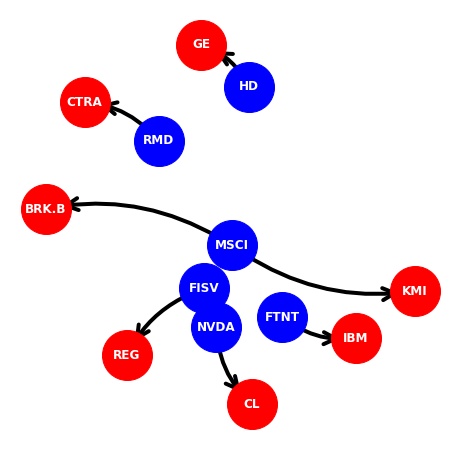
\includegraphics[width=\linewidth]{bullNetwork.png}
        \caption{Bull market lead-lag pairs.}
        \label{fig:bullNetwork}
    \end{subfigure}
    \hfill
    \begin{subfigure}{0.45\textwidth}
        \centering
        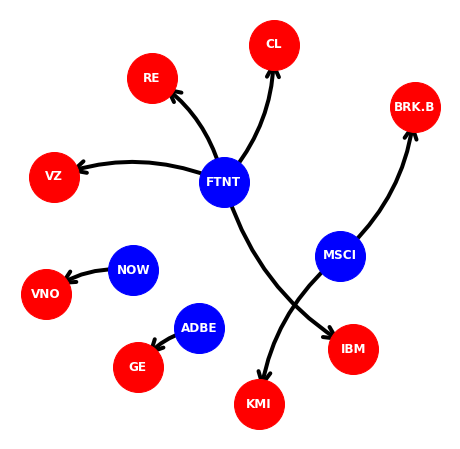
\includegraphics[width=\linewidth]{bearNetwork.png}
        \caption{Bear market lead-lag pairs.}
        \label{fig:bearNetwork}
    \end{subfigure}
    \caption{Network graphs of lead-lag pairs for the first day of trading. Blue nodes represent laggers with directed edges connected them to red nodes representing leaders.}
    \label{fig:networks}
\end{figure}
\subsection{Portfolio Returns and Parameter Exploration}
Over the course of the last four fiscal quarters and during the summer of 2021, our portfolio, see Fig. \ref{fig:portfolio}\footnote{Using the optimal values of buying threshold and trailing stop percentage.} returns mirrored the ebb and flow of the S$\&$P 500's history. During a bear market our portfolio does not experience positive growth during the same period, in fact, we loose roughly five percent in value while the S$\&$P 500 approximately looses fifteen percent, see Fig. \ref{fig:bearPlot}.\footnote{Hence, someone who did not invest at all would have kept the value of their capital while our portfolio and the S$\&$P 500's value diminished, not account for inflation} Moreover, during a bull market, we observe a positive return roughly two percent greater than the S$\&$P 500 during the same period, see Fig. \ref{fig:bullPlot}.
\begin{figure}[H]
    \centering
    \begin{subfigure}{0.495\textwidth}
        \centering
        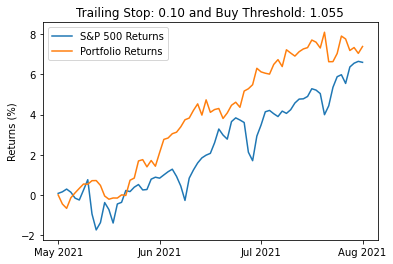
\includegraphics[width=\linewidth]{bullPlot.png}
        \caption{Bull market of Q2 and Q3 of 2021.}
        \label{fig:bullPlot}
    \end{subfigure}
    \hfill
    \begin{subfigure}{0.495\textwidth}
        \centering
        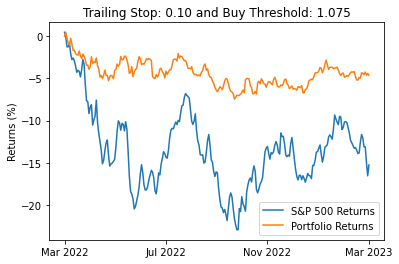
\includegraphics[width=\linewidth]{bearPlot.png}
        \caption{Bear market of the past four quarters.}
        \label{fig:bearPlot}
    \end{subfigure}
    \caption{Back-testing of portfolio returns compared to historical returns of the S$\&$P 500  ($^\wedge$GSPC).}
    \label{fig:portfolio}
\end{figure}
Naturally, we were prompted to conduct basic parameter exploration with the hopes of maximizing our return given our risk preferences amongst other variables. In Fig. \ref{fig:contourPlot}, we explore the portfolio return, buy threshold, and trailing stop percentage parameter space.
%I believe it is more insightful to see trailing stop percentage held constant, which is not the case in 3b, where buy threshold is being held constant.
\begin{figure}[H]
    \centering
    \begin{subfigure}{0.495\textwidth}
        \centering
        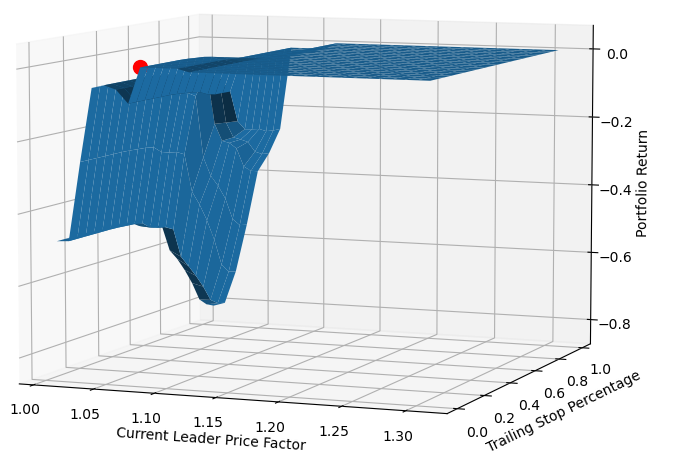
\includegraphics[width=\linewidth]{contourPlot.png}
        \caption{Contour plot.}
        \label{fig:contourPlot}
    \end{subfigure}
    \hfill
    \begin{subfigure}{0.495\textwidth}
        \centering
        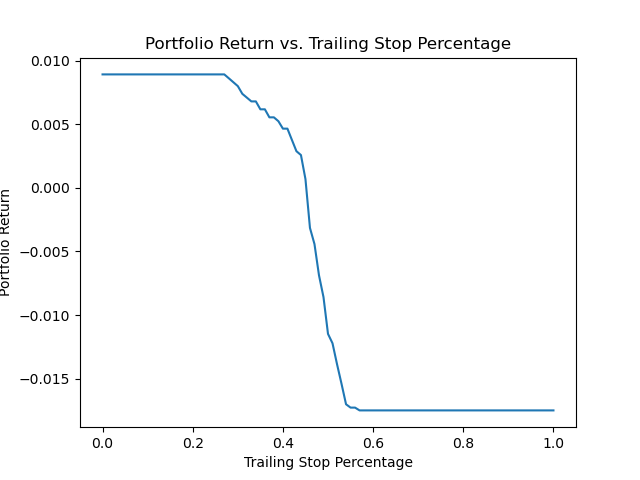
\includegraphics[width=\linewidth]{slicePlot.png}
        \caption{2D cross-section of contour plot, holding trailing stop percentage constant.}
        \label{fig:slicePlot}
    \end{subfigure}
    \caption{Mesh grid plot of trailing stop percentage vs. buy threshold vs. portfolio returns}
    \label{fig:parameters}
\end{figure}
\section{Code hurdles}
%Kevin
Talk about data collection and processing
Include notes from slides
Etc.
\section{Analysis and Conclusions}
%Jonah
\section{Considerations and Future work}
%Aarush
\section*{References}
[1]: Li, Y., Wang, T., Sun, B., \& Liu. Detecting the lead–lag effect in stock markets: Definition, patterns, and investment strategies. Financial Innovation, 2022.

[2]: A. Namaki, A.H. Shirazi, R. Raei, and G.R. Jafari. Network analysis of a financial market based on genuine correlation and threshold method. Physica A: Statistical
Mechanics and its Applications, 2011.

[3]: R. D. Smith. The Spread of the Credit Crisis: View
from a Stock Correlation Network. Journal of Korean
Physical Society, 54:2460, June 2009.

\medskip
\small
\end{document}
